% Required packages: pgfplots, lmodern
% Required TikZ libraries: none
% Target width: 160 mm maximum
% Minimum text size: 9 pt
% Colour/greyscale intent: colour_and_greyscale, direct labels and line styles
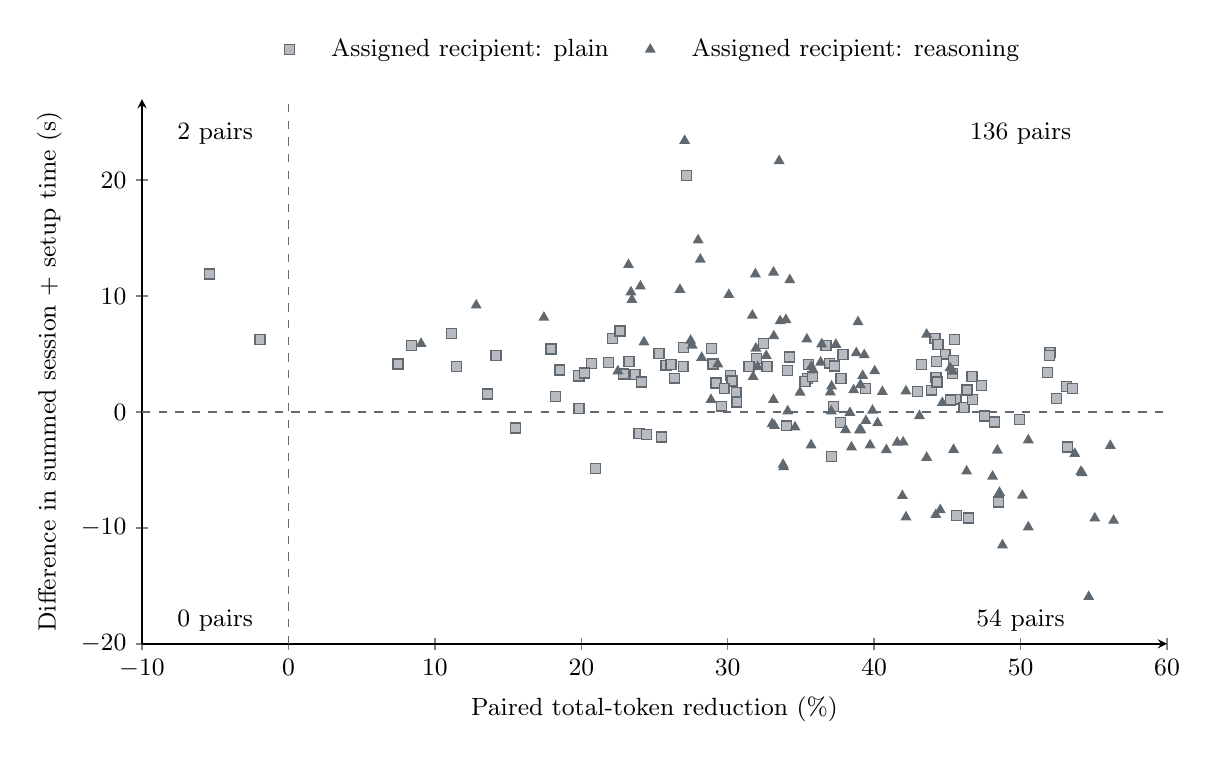
\begin{tikzpicture}
\definecolor{ealblue}{HTML}{165D81}
\definecolor{ordinaryorange}{HTML}{C27021}
\definecolor{neutralgrey}{HTML}{616970}
\pgfplotsset{compat=1.18,
  every axis/.append style={
    width=148mm,height=66mm,
    font=\fontsize{9}{11}\selectfont,
    tick label style={font=\fontsize{9}{11}\selectfont},
    label style={font=\fontsize{9}{11}\selectfont},
    title style={font=\fontsize{10}{12}\selectfont},
    legend style={font=\fontsize{9}{11}\selectfont,draw=none,fill=none},
    axis lines=left,axis line style={line width=0.5pt},
    tick style={line width=0.5pt},
    grid style={line width=0.4pt,black!12},
    scaled ticks=false,clip=false}}
\begin{axis}[width=146mm,height=85mm,xmin=-10,xmax=60,ymin=-20,ymax=27,xtick={-10,0,10,20,30,40,50,60},ytick={-20,-10,0,10,20},xlabel={Paired total-token reduction (\%)},ylabel={Difference in summed session + setup time (s)},legend columns=2,legend style={at={(0.5,1.05)},anchor=south,column sep=4mm}]
\addplot[forget plot,neutralgrey,dashed,line width=0.5pt,no marks] coordinates {(0,-20) (0,27)};
\addplot[forget plot,neutralgrey,dashed,line width=0.5pt,no marks] coordinates {(-10,0) (60,0)};
\addplot[only marks,mark=square*,mark size=1.8pt,neutralgrey,line width=0.5pt,mark options={fill=neutralgrey!45}] coordinates {(25.47589397,-2.163701613) (45.49911338,6.257343742) (11.46252545,3.915675499) (25.78910776,4.038094831) (37.71578947,-0.917661715) (30.57637632,1.693360746) (45.60041408,1.1039367) (36.93105002,4.210404886) (47.32106753,2.282870861) (45.21614423,1.032325238) (23.67439598,3.213211294) (30.18468059,3.127383364) (7.473908097,4.147215549) (-1.948890761,6.257474585) (21.84600157,4.274778401) (20.95952448,-4.892470915) (43.22568671,4.089681934) (48.20556024,-0.877525533) (22.12123848,6.329948445) (30.6188364,0.86123415) (23.94515197,-1.879606107) (37.07577612,-3.846525598) (46.43051771,-9.133382076) (45.63146159,-8.932867727) (48.47703145,-7.761638205) (36.7198666,5.747249396) (44.15694392,6.35188986) (24.44644464,-1.949000744) (53.12167435,2.223348985) (39.42517584,2.051869019) (31.96887091,4.609919938) (46.1368865,0.377039366) (35.45502367,2.90370482) (44.84872069,4.986862961) (51.99892675,5.129511189) (22.6534603,6.990713101) (26.98917887,5.580315455) (35.28163785,2.606456488) (37.74410415,2.897239366) (53.19662244,-3.015354455) (44.35739786,5.804833537) (19.85340127,3.097758515) (17.92354671,5.448690078) (53.53934603,2.046908021) (31.44165155,3.901274282) (22.86242366,3.280008709) (19.84912777,0.290083635) (29.56521739,0.502267194) (43.91499719,1.879559221) (27.19420089,20.41796987) (51.83103698,3.414917005) (19.8066425,3.142739855) (51.9622811,4.876396815) (37.27796153,3.957719612) (26.36032931,2.916551517) (35.78160546,3.043797281) (44.23981993,4.359206068) (11.13300019,6.758918079) (44.2169238,2.985069437) (44.28017002,2.57759099) (28.98289179,4.146321847) (-5.383882003,11.89107135) (13.58637986,1.556525325) (30.2852149,2.671242594) (34.02493975,-1.190420943) (45.40522947,4.420405028) (37.24025974,0.4718182) (52.44531389,1.1608373) (29.2056991,2.490527287) (26.95640813,3.936240358) (23.25791078,4.366682596) (32.68701113,3.947861706) (34.21295229,4.738910607) (35.50017228,4.100624567) (42.96752829,1.763497908) (25.31592641,5.055457256) (15.51088933,-1.382855518) (18.24857221,1.313938288) (46.71712007,1.093335337) (26.12170995,4.110382908) (20.68727336,4.189875211) (49.91268917,-0.646392037) (24.12980789,2.579930953) (45.35999192,3.311217677) (8.39323878,5.724769313) (28.87773554,5.490251956) (47.52542952,-0.345442532) (20.20821449,3.363960936) (18.53107345,3.621839159) (34.09066437,3.601485953) (29.75799223,2.044466445) (37.86707883,4.984463616) (46.68513957,3.044567545) (32.44843131,5.920199708) (46.33528265,1.896307104) (14.17611898,4.875890855)};
\addlegendentry{Assigned recipient: plain}
\addplot[only marks,mark=triangle*,mark size=1.8pt,neutralgrey,line width=0.5pt,mark options={fill=neutralgrey}] coordinates {(27.57172223,5.747234013) (17.44628535,8.153306981) (56.12734864,-2.909942854) (24.0374426,10.84390623) (35.7070331,3.925607451) (39.43536404,-0.760917581) (35.40425532,6.278978397) (36.34389276,4.285328397) (37.00541783,1.712627485) (33.57746904,7.851632518) (44.65242502,0.793227413) (33.96938562,7.951545512) (50.52448474,-9.932111153) (34.93900532,1.694824291) (48.08639267,-5.557344284) (33.14747919,6.552886857) (56.35041738,-9.365241563) (28.85457295,1.057636053) (34.23909593,11.39089786) (38.0445835,-1.544513148) (43.0912541,-0.33570327) (22.49891325,3.52490521) (31.6812521,8.333064133) (33.12820513,12.05030462) (32.04410117,3.882535062) (33.8183978,-4.739298292) (34.09728718,0.075732349) (39.32177425,4.927154781) (53.69670804,-3.594064904) (40.03317467,3.531721781) (27.05748733,23.40844448) (45.42368914,-3.250407929) (43.58321203,6.690627101) (54.11594801,-5.148155175) (41.5721888,-2.623002243) (27.46369082,6.168986069) (38.34306957,-0.06335573) (40.23020579,-0.95468713) (29.32226833,4.125228423) (31.92439588,5.490270877) (45.37082717,3.50514843) (38.77973113,5.095334968) (48.55738653,-6.952903846) (30.0738494,10.11459188) (40.83228048,-3.270402303) (50.52454204,-2.42226147) (33.19264611,-1.185035184) (32.63053042,4.850203565) (38.59589041,1.893191449) (39.88584755,0.131050104) (38.99296557,-1.573349319) (35.69420169,-2.854230646) (38.44914542,-3.034977795) (31.73352017,3.036349952) (46.31536713,-5.116078168) (43.58634174,-3.933080573) (50.12229923,-7.205101627) (37.06877609,0.068466275) (28.12731997,13.1590717) (23.38895282,10.34041111) (28.21856882,4.691874769) (54.65019494,-15.94272586) (33.03360151,-1.026182857) (39.05899925,2.337698772) (31.88696597,11.89748402) (33.51136884,21.66339772) (39.21351426,3.13090609) (40.5605174,1.750618472) (48.41148724,-3.307158952) (33.77797216,-4.53540559) (42.17337582,-9.067906908) (41.981235,-2.609195684) (9.055690073,5.901342715) (37.38417384,5.814249869) (12.82220269,9.208129044) (35.82913757,3.604167627) (23.4546067,9.680892035) (48.7599977,-11.48390383) (26.73630948,10.55780324) (44.51060662,-8.448241529) (41.92673816,-7.231470037) (39.71995632,-2.859519142) (37.09214502,2.220513374) (45.18181818,3.80231422) (39.08678982,-1.542789149) (54.20688356,-5.259894141) (24.27808379,6.030446082) (42.17005909,1.800895549) (23.2234315,12.69917293) (27.97565923,14.82507364) (44.21003282,-8.868196331) (38.89681408,7.769877705) (36.41430948,5.854624442) (34.59489994,-1.312543858) (55.06320511,-9.170126744) (33.11853577,1.058943187)};
\addlegendentry{Assigned recipient: reasoning}
\node[font=\fontsize{9}{11}\selectfont] at (axis cs:-5,24) {2 pairs};
\node[font=\fontsize{9}{11}\selectfont] at (axis cs:50,24) {136 pairs};
\node[font=\fontsize{9}{11}\selectfont] at (axis cs:-5,-18) {0 pairs};
\node[font=\fontsize{9}{11}\selectfont] at (axis cs:50,-18) {54 pairs};
\end{axis}
\end{tikzpicture}
